% Environment -> welfare -> human activity feedback loop.
% Compile to SVG:  latex valuation_cycle.tex && dvisvgm --no-fonts valuation_cycle.dvi -o ../valuation_cycle.svg
\documentclass[tikz,border=6pt]{standalone}
\usepackage[scaled]{helvet}
\renewcommand{\familydefault}{\sfdefault}
\usetikzlibrary{arrows.meta}
\definecolor{accent}{HTML}{2E7D32}
\begin{document}
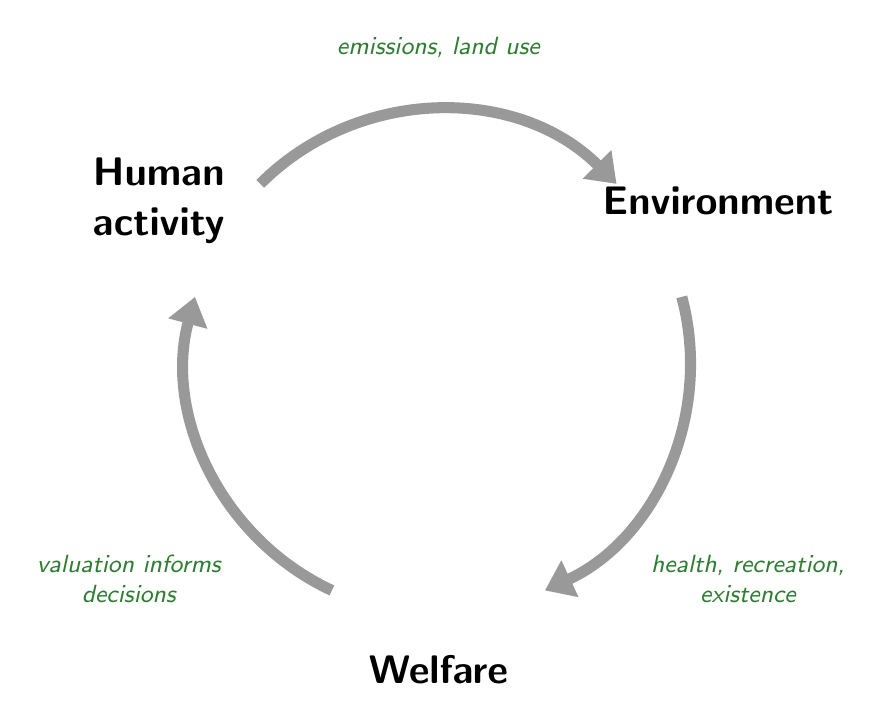
\begin{tikzpicture}[
    loop/.style={line width=4pt, draw=black!40, -{Triangle[length=10pt,width=14pt]}},
    node/.style={font=\Large\bfseries, align=center},
    lab/.style={font=\small\itshape, text=accent, align=center}]
  \def\R{3.2}
  \node[node] at (150:\R+0.9) {Human\\activity};
  \node[node] at ( 30:\R+0.9) {Environment};
  \node[node] at (270:\R+0.7) {Welfare};
  % arcs (counter-clockwise angles, drawn clockwise)
  \draw[loop] (135:\R) arc[start angle=135, end angle=45,  radius=\R];
  \draw[loop] ( 15:\R) arc[start angle=15,  end angle=-65, radius=\R];
  \draw[loop] (245:\R) arc[start angle=245, end angle=165, radius=\R];
  \node[lab] at ( 90:\R+0.8) {emissions, land use};
  \node[lab] at (-35:\R+1.6) {health, recreation,\\existence};
  \node[lab] at (215:\R+1.6) {valuation informs\\decisions};
\end{tikzpicture}
\end{document}
